% 原書231--255頁（PDF253--277）、第8章導入および8.1--8.4。
\sectionlink{トーラスコンパクト化と \texorpdfstring{$T$}{T} 双対性}\label{ch:8}

弦理論の現実的なコンパクト化は第2巻の後半の章で扱うが、一つ以上の次元を周期的に同一視する、弦理論の最も簡単なコンパクト化をここで見ておくのは興味深い。まず場の理論における同じコンパクト化を考え、特にゲージ相互作用と重力の Kaluza--Klein 統一に出会う。次にこれを弦理論へ拡張する。そこでは、巻き付き状態、拡大されたゲージ対称性、$T$ 双対性、Dブレーンという、いくつかの新しい、弦に本質的な現象が生じる。また、少し複雑なコンパクト化であるオービフォールドとオリエンティフォールドも考えることになる。

\subsectionlink{場の理論におけるトーラスコンパクト化}\label{sec:8.1}

一般相対論では、時空の幾何は力学的である。私たちが見る三つの空間次元は膨張しており、かつては大きく曲がっていた。小さいままの余分な次元が存在するというのは、論理的に可能である。実際、電磁場と重力場を単一の高次元の場の成分として統一する方法として、この考えは早くも1914年に提案されていた。$x^4$ が周期的で、
\begin{equation}
x^4\cong x^4+2\pi R,
\tag{8.1.1}\label{eq:8.1.1}
\end{equation}
$\mu=0,\ldots,3$ に対する $x^\mu$ が非コンパクトな5次元理論を考える。これが\emph{トーラスコンパクト化}である。5次元計量は $G_{\mu\nu}$、$G_{\mu4}$、$G_{44}$ に分かれる。4次元の観点からは、これらは計量、ベクトル、スカラーである。

より一般に、$x^d$ が周期的な $D=d+1$ 時空次元の場合を取り、詳しく見てみよう。まだ場の理論を考えているので、$D$ は任意のままとする。計量を
\begin{equation}
ds^2=G^D_{MN}dx^Mdx^N=G_{\mu\nu}dx^\mu dx^\nu
+G_{dd}(dx^d+A_\mu dx^\mu)^2
\tag{8.1.2}\label{eq:8.1.2}
\end{equation}
とパラメータ表示する。添字 $M,N$ はすべての次元 $0,\ldots,d$ を走り、添字 $\mu,\nu$ は非コンパクトな次元 $0,\ldots,d-1$ だけを走る。完全な $D$ 次元計量を $G^D_{MN}$ と表す。$G_{\mu\nu}\ne G^D_{\mu\nu}$ であることに注意しよう。$d$ 次元の作用では、$G_{\mu\nu}$ を用いて添字を上げ下げする。今のところ、場 $G_{\mu\nu}$、$G_{dd}$、$A_\mu$ は非コンパクト座標 $x^\mu$ だけに依存してよいものとする。形 \hyperref[eq:8.1.2]{(8.1.2)} は、$x^d$ の並進のもとで不変な最も一般的な計量である。この形でも、$d$ 次元の再パラメータ化 $x'^\mu(x^\nu)$ と、再パラメータ化
\begin{equation}
x'^d=x^d+\lambda(x^\mu)
\tag{8.1.3}\label{eq:8.1.3}
\end{equation}
が許される。後者のもとでは
\begin{equation}
A'_\mu=A_\mu-\partial_\mu\lambda
\tag{8.1.4}\label{eq:8.1.4}
\end{equation}
なので、ゲージ変換が高次元の座標変換群の一部として現れる。これが \emph{Kaluza--Klein 機構}である。

$x^d$ 依存性の効果を見るため、$D$ 次元の質量ゼロのスカラー $\phi$ を考える。簡単のため、コンパクト方向の計量を $G_{dd}=1$ とする。周期的な次元の運動量は $p_d=n/R$ と量子化される。$\phi$ の $x^d$ 依存性を完全系で展開すると、
\begin{equation}
\phi(x^M)=\sum_{n=-\infty}^{\infty}\phi_n(x^\mu)\exp(inx^d/R).
\tag{8.1.5}\label{eq:8.1.5}
\end{equation}
$D$ 次元の波動方程式 $\partial_M\partial^M\phi=0$ は
\begin{equation}
\partial_\mu\partial^\mu\phi_n(x^\mu)=\frac{n^2}{R^2}\phi_n(x^\mu)
\tag{8.1.6}\label{eq:8.1.6}
\end{equation}
となる。したがって $D$ 次元の場のモード $\phi_n$ は、$n$ でラベルされる $d$ 次元の場の無限の塔になる。$d$ 次元の質量の二乗
\begin{equation}
-p^\mu p_\mu=\frac{n^2}{R^2}
\tag{8.1.7}\label{eq:8.1.7}
\end{equation}
は、$p_d$ がゼロでないすべての場についてゼロでない。$R^{-1}$ より十分低いエネルギーでは、$x^d$ に依存しない場だけが残り、物理は $d$ 次元になる。$R^{-1}$ より高いエネルギーでは、Kaluza--Klein 状態の塔が見える。

Kaluza--Klein ゲージ不変性 \hyperref[eq:8.1.3]{(8.1.3)} に対応する電荷は、運動量 $p_d$ である。この簡単な例では、Kaluza--Klein 電荷を持つすべての場に質量がある。より一般には、高スピンの場と曲がった背景があると、質量ゼロの荷電場が存在しうる。

質量ゼロの場の有効作用は、常に考察すべき重要な対象である。$G_{dd}=e^{2\sigma}$ と定義する。計量 \hyperref[eq:8.1.2]{(8.1.2)} の Ricci スカラーは
\begin{equation}
\bm R=\bm R_d-2e^{-\sigma}\nabla^2e^\sigma-\frac14e^{2\sigma}F_{\mu\nu}F^{\mu\nu},
\tag{8.1.8}\label{eq:8.1.8}
\end{equation}
ただし $\bm R$ は $G^D_{MN}$ から、$\bm R_d$ は $G_{\mu\nu}$ から構成する。重力子・ディラトン作用 \hyperref[eq:3.7.20]{(3.7.20)} は
\begin{equation}
\begin{aligned}
\bm S_1&=\frac1{2\kappa_0^2}\int d^Dx\,(-G_D)^{1/2}e^{-2\Phi}
(\bm R+4\nabla_\mu\Phi\nabla^\mu\Phi)\\
&=\frac{\pi R}{\kappa_0^2}\int d^dx\,(-G_d)^{1/2}e^{-2\Phi+\sigma}\\
&\qquad\times\left(\bm R_d-4\partial_\mu\Phi\partial^\mu\sigma
+4\partial_\mu\Phi\partial^\mu\Phi-\frac14e^{2\sigma}F_{\mu\nu}F^{\mu\nu}\right)\\
&=\frac{\pi R}{\kappa_0^2}\int d^dx\,(-G_d)^{1/2}e^{-2\Phi_d}\\
&\qquad\times\left(\bm R_d-\partial_\mu\sigma\partial^\mu\sigma
+4\partial_\mu\Phi_d\partial^\mu\Phi_d-\frac14e^{2\sigma}F_{\mu\nu}F^{\mu\nu}\right)
\end{aligned}
\tag{8.1.9}\label{eq:8.1.9}
\end{equation}
となり、すべての質量ゼロの場の運動項を与える。ここで $G_d$ は $G_{\mu\nu}$ の行列式を表し、最後の行では有効な $d$ 次元ディラトン $\Phi_d=\Phi-\sigma/2$ を導入した。ディラトンの運動項の符号が誤っているように見えるのは見かけだけである。重力子と計量のトレースとの混合も考慮する必要があるからだ。これは式 \hyperref[eq:3.7.25]{(3.7.25)} のような Weyl 変換によって最も簡単に扱え、得られる運動項は正しい符号を持つ。

場の方程式は、コンパクトな次元の半径を決めない。\footnote[1]{もちろん、物理的に非同値な解を区別するのは、不変な半径
\[
\rho=Re^\sigma
\]
だけである。$R$ を、たとえば $\alpha'^{1/2}$ のような便利な値に、あるいは無次元変数を使うなら1に固定してもよいが、一般のままにしておくと便利である。しばしば、代わりに $G_{dd}$ を1に固定する方が便利である。同様に、$\Phi$ を加法的にシフトして、$\kappa_0^2$ を $\alpha'$ の適切なべきに固定することもできるが、ここでも一般のままにしておいて支障はない。第13章では、$\Phi$ の加法的な規格化を別の方法で固定するのが自然であることを見る。}平坦な計量と定数のディラトンは、$\Phi$ と $\sigma$ の任意の値について解である。言い換えれば、$\Phi$ にも $\sigma$ にもポテンシャルエネルギーはなく、したがってこれらの場は、Goldstone ボソンとよく似て質量ゼロである。$\Phi$ と $\sigma$ の異なる値は、縮退した配位（量子論では状態）をラベルし、これらの場がゆっくり変化する状態では、エネルギーは勾配だけから生じる。Goldstone 現象との違いは、縮退した状態がいかなる対称性によっても互いに関係づけられておらず、実際に物理が $\Phi$ と $\sigma$ に依存することである。このボース理論では縮退は偶然であり、前章で議論した1ループのエネルギーが縮退を破る。超対称理論では、物理的に非同値でありながら縮退した真空の存在はごく一般的であり、力学の理解に重要な役割を果たす。非同値な真空をラベルするこれらの質量ゼロの場は、\emph{モジュライ}と呼ばれる。自然界では、超対称性の破れがほぼ確実にすべてのモジュライに質量を与えなければならない。そうでなければ、これらはほぼ重力程度の強さで無限の到達距離を持つ相互作用を媒介してしまう。第14章では、ある弦理論において、ディラトン自身が、弦の摂動論では明らかでない隠れた次元の半径であることを見る。

$A_\mu=R\widetilde A_\mu$ と定義すると、共変微分は
\begin{equation}
\partial_\mu+ip_dA_\mu=\partial_\mu+in\widetilde A_\mu
\tag{8.1.10}\label{eq:8.1.10}
\end{equation}
となり、電荷は整数になる。$d$ 次元のゲージ結合と重力結合は、通常、次のように定義する。Lagrangian 密度の $\widetilde F_{\mu\nu}\widetilde F^{\mu\nu}$ の係数を $-1/(4g_d^2)$、$\bm R_d$ の係数を $1/(2\kappa_d^2)$ と定義する。したがってゲージ結合は、重力結合によって
\begin{equation}
g_d^2=\frac{\kappa_0^2e^{2\Phi_d}}{\pi R^3e^{2\sigma}}
=\frac{2\kappa_d^2}{\rho^2}
\tag{8.1.11}\label{eq:8.1.11}
\end{equation}
と決まる。$d$ 次元と $D$ 次元の重力結合は
\begin{equation}
\frac1{\kappa_d^2}=\frac{2\pi\rho}{\kappa^2}
\tag{8.1.12}\label{eq:8.1.12}
\end{equation}
で関係づけられ、$2\pi\rho$ はコンパクト化された次元の体積である。

反対称テンソルも、Kaluza--Klein 機構の一般化によってゲージ対称性を生む。$B_{MN}$ を $B_{\mu\nu}$ と $A'_\mu=B_{d\mu}$ に分けると、式 \hyperref[eq:3.7.7]{(3.7.7)} で定義したゲージパラメータ $\zeta_M$ は、$d$ 次元の反対称テンソル変換 $\zeta_\mu$ と、通常のゲージ不変性 $\zeta_d$ に分かれる。ゲージ場は $B_{d\mu}$、場の強さは $H_{d\mu\nu}$ である。反対称テンソルの作用は
\begin{equation}
\begin{aligned}
\bm S_2&=-\frac1{24\kappa_0^2}\int d^Dx\,(-G_D)^{1/2}e^{-2\Phi}H_{MNL}H^{MNL}\\
&=-\frac{\pi R}{12\kappa_0^2}\int d^dx\,(-G_d)^{1/2}e^{-2\Phi_d}
\left(\widetilde H_{\mu\nu\lambda}\widetilde H^{\mu\nu\lambda}
+3e^{-2\sigma}H_{d\mu\nu}H_d{}^{\mu\nu}\right)
\end{aligned}
\tag{8.1.13}\label{eq:8.1.13}
\end{equation}
となる。ここで
\begin{equation}
\widetilde H_{\mu\nu\lambda}=(\partial_\mu B_{\nu\lambda}-A_\mu H_{d\nu\lambda})
+\text{巡回置換項}
\tag{8.1.14}\label{eq:8.1.14}
\end{equation}
と定義した。ベクトルポテンシャルに比例する項は、逆計量 $G^{MN}$ から生じる。これは \emph{Chern--Simons 項}と呼ばれる。この名称は、一つのゲージポテンシャルと任意個の場の強さを反対称化して組み合わせたものを意味する。このような項は超対称理論のさまざまな場所に現れ、興味深い物理的効果と結び付いている。特に、$A_\mu$ の変換 \hyperref[eq:8.1.4]{(8.1.4)} が、変換
\begin{equation}
B'_{\nu\lambda}=B_{\nu\lambda}-\lambda H_{d\nu\lambda}
\tag{8.1.15}\label{eq:8.1.15}
\end{equation}
によって相殺されるため、$\widetilde H_{\mu\nu\lambda}$ がゲージ不変であることに注意しよう。

ポテンシャル $B_{MN}$ を他の場に最小結合させる方法はない。したがって Kaluza--Klein の場合とは異なり、反対称テンソルのゲージ対称性のもとで電荷を持つ場は存在しない。この点は弦理論では異なる。

\subsectionlink{CFT におけるトーラスコンパクト化}\label{sec:8.2}

次に、一つの周期的なスカラー場
\begin{equation}
X\cong X+2\pi R
\tag{8.2.1}\label{eq:8.2.1}
\end{equation}
の共形場理論を考える。式を煩雑にしないため、$X^d$ の上添字を省き、$G_{dd}=1$ と置く。世界面の作用は非コンパクトな理論と同じ $\int d^2z\,\partial X\bar\partial X/(2\pi\alpha')$ なので、運動方程式、演算子積、エネルギー運動量テンソルは変わらない。特に、この理論は依然として共形不変である。周期性には二つの効果がある。第一に、弦の状態は同一視 \hyperref[eq:8.2.1]{(8.2.1)} のもとで一価でなければならない。すなわち、周期的な次元を一周するよう弦を並進させる演算子 $\exp(2\pi iRp)$ は状態を不変に保たなければならないので、重心運動量が
\begin{equation}
k=\frac nR,\qquad n\in\mathbb Z
\tag{8.2.2}\label{eq:8.2.2}
\end{equation}
と量子化される。これは場の理論と同じである。

第二の効果は弦理論に特有である。今度は閉弦がコンパクト方向に巻き付くことができる：
\begin{equation}
X(\sigma+2\pi)=X(\sigma)+2\pi Rw,\qquad w\in\mathbb Z.
\tag{8.2.3}\label{eq:8.2.3}
\end{equation}
整数 $w$ は\emph{巻き付き数}である。巻き付き数 $+1$、$0$、$-1$ の状態を図\ref{fig:8.1}(a) に示した。世界面の場の理論の観点からは、巻き付き数がゼロでない弦は、位相的に非自明な場の配位を持つ状態、すなわち\emph{位相的ソリトン}である。整合的な弦理論は、巻き付き数を持つ状態を含まなければならない。図\ref{fig:8.1}(b) のように、通常の分裂・結合過程によって、$w=0$ の弦が $w=+1$ と $w=-1$ の対に変わりうるからである。この例のように、巻き付き数が常に保存することは容易に分かる。

\begin{figure}[htbp]
\centering
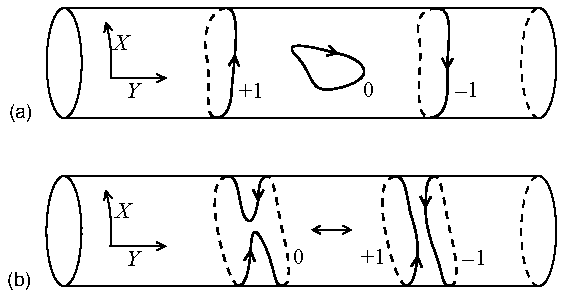
\includegraphics[width=0.9\linewidth]{figures/fig_8_1.pdf}
\caption{(a) 巻き付き数 $w=+1,0,-1$ の向き付き閉弦。説明のため、コンパクトな次元 $X$ を一つ、非コンパクトな次元 $Y$ を一つ示している。(b) $w=0$ の弦から、$w=+1$ および $w=-1$ の弦への遷移。}\label{fig:8.1}
\end{figure}

閉弦 CFT の状態を記述するため、Laurent 展開
\begin{equation}
\partial X(z)=-i\left(\frac{\alpha'}2\right)^{1/2}\sum_{m=-\infty}^{\infty}\frac{\alpha_m}{z^{m+1}},
\qquad
\bar\partial X(\bar z)=-i\left(\frac{\alpha'}2\right)^{1/2}\sum_{m=-\infty}^{\infty}\frac{\widetilde\alpha_m}{\bar z^{m+1}}
\tag{8.2.4}\label{eq:8.2.4}
\end{equation}
を考える。弦を一周するときの座標 $X$ の全変化は
\begin{equation}
2\pi Rw=\oint(dz\,\partial X+d\bar z\,\bar\partial X)
=2\pi(\alpha'/2)^{1/2}(\alpha_0-\widetilde\alpha_0).
\tag{8.2.5}\label{eq:8.2.5}
\end{equation}
全 Noether 運動量は
\begin{equation}
p=\frac1{2\pi\alpha'}\oint(dz\,\partial X-d\bar z\,\bar\partial X)
=(2\alpha')^{-1/2}(\alpha_0+\widetilde\alpha_0).
\tag{8.2.6}\label{eq:8.2.6}
\end{equation}
非コンパクトな次元なら、通常の関係 $\alpha_0=\widetilde\alpha_0=p(\alpha'/2)^{1/2}$ が得られるが、周期的な次元では
\begin{align}
p_L&\equiv(2/\alpha')^{1/2}\alpha_0=\frac nR+\frac{wR}{\alpha'},
\tag{8.2.7a}\label{eq:8.2.7a}\\
p_R&\equiv(2/\alpha')^{1/2}\widetilde\alpha_0=\frac nR-\frac{wR}{\alpha'}.
\tag{8.2.7b}\label{eq:8.2.7b}
\end{align}
Virasoro 生成子は
\begin{align}
L_0&=\frac{\alpha'p_L^2}4+\sum_{n=1}^{\infty}\alpha_{-n}\alpha_n,
\tag{8.2.8a}\label{eq:8.2.8a}\\
\widetilde L_0&=\frac{\alpha'p_R^2}4+\sum_{n=1}^{\infty}\widetilde\alpha_{-n}\widetilde\alpha_n.
\tag{8.2.8b}\label{eq:8.2.8b}
\end{align}

\subsubsectionlink*{分配関数}

$X$ の分配関数は今度は
\begin{equation}
\begin{aligned}
(q\bar q)^{-1/24}\operatorname{Tr}(q^{L_0}\bar q^{\widetilde L_0})
&=|\eta(\tau)|^{-2}\sum_{n,w=-\infty}^{\infty}
q^{\alpha'p_L^2/4}\bar q^{\alpha'p_R^2/4}\\
&=|\eta(\tau)|^{-2}\sum_{n,w=-\infty}^{\infty}
\exp\left[-\pi\tau_2\left(\frac{\alpha'n^2}{R^2}+\frac{w^2R^2}{\alpha'}\right)+2\pi i\tau_1nw\right].
\end{aligned}
\tag{8.2.9}\label{eq:8.2.9}
\end{equation}
振動子の和は非コンパクトな場合と同じだが、運動量積分は $n$ と $w$ の和に置き換わる。モジュラー不変性は明白ではないが、Poisson 再総和公式
\begin{equation}
\sum_{n=-\infty}^{\infty}\exp(-\pi an^2+2\pi ibn)
=a^{-1/2}\sum_{m=-\infty}^{\infty}\exp\left[-\frac{\pi(m-b)^2}{a}\right]
\tag{8.2.10}\label{eq:8.2.10}
\end{equation}
を使えば明白にできる。分配関数は
\begin{equation}
2\pi RZ_X(\tau)\sum_{m,w=-\infty}^{\infty}
\exp\left(-\frac{\pi R^2|m-w\tau|^2}{\alpha'\tau_2}\right)
\tag{8.2.11}\label{eq:8.2.11}
\end{equation}
となる。ここで $Z_X(\tau)$ は非コンパクトな理論のモジュラー不変な表式 \hyperref[eq:7.2.9]{(7.2.9)} である。変数を $m\to m+w$ と変えれば、この和は明らかに $\tau\to\tau+1$ のもとで不変である。また、$m\to-w$、$w\to m$ とすれば、$\tau\to-1/\tau$ のもとでも不変である。

表式 \hyperref[eq:8.2.11]{(8.2.11)} には簡単な経路積分による解釈がある。周期的な時空で種数1のすべての世界面について和を取るとき、世界面上の各非自明な閉曲線はコンパクト方向に巻き付くことができる：
\begin{align}
X(\sigma^1+2\pi,\sigma^2)&=X(\sigma^1,\sigma^2)+2\pi wR,
\tag{8.2.12a}\label{eq:8.2.12a}\\
X(\sigma^1+2\pi\tau_1,\sigma^2+2\pi\tau_2)&=X(\sigma^1,\sigma^2)+2\pi mR.
\tag{8.2.12b}\label{eq:8.2.12b}
\end{align}
すなわち、経路積分は $w$ と $m$ でラベルされる位相的に異なるセクターに分かれる。Gaussian 経路積分は、$X$ を正しい周期性を持つ古典解
\begin{equation}
X_{\mathrm{cl}}=\sigma^1wR+\sigma^2(m-w\tau_1)R/\tau_2
\tag{8.2.13}\label{eq:8.2.13}
\end{equation}
と、周期境界条件を満たす量子的な部分との和として書く、通常の方針で実行できる。作用は古典的な部分と量子的な部分に分かれる。量子的な部分の経路積分は非コンパクトな場合と同じであり、古典作用は式 \hyperref[eq:8.2.11]{(8.2.11)} の指数に現れる。このとき、モジュラー変換が周期性に及ぼす効果は、単に和の変数 $m,w$ の変更となる。

\subsubsectionlink*{頂点演算子}

$\alpha_0\ne\widetilde\alpha_0$ となる巻き付き状態を作るには、
\begin{equation}
[x_L,p_L]=[x_R,p_R]=i
\tag{8.2.14}\label{eq:8.2.14}
\end{equation}
を満たす独立な変数 $x_L,x_R$ が必要である。このとき場 $X$ は正則部分と反正則部分に分かれる：
\begin{equation}
X(z,\bar z)=X_L(z)+X_R(\bar z),
\tag{8.2.15}\label{eq:8.2.15}
\end{equation}
ただし
\begin{align}
X_L(z)&=x_L-i\frac{\alpha'}2p_L\ln z
+i\left(\frac{\alpha'}2\right)^{1/2}\sum_{\substack{m=-\infty\\m\ne0}}^{\infty}\frac{\alpha_m}{mz^m},
\tag{8.2.16a}\label{eq:8.2.16a}\\
X_R(\bar z)&=x_R-i\frac{\alpha'}2p_R\ln\bar z
+i\left(\frac{\alpha'}2\right)^{1/2}\sum_{\substack{m=-\infty\\m\ne0}}^{\infty}\frac{\widetilde\alpha_m}{m\bar z^m}.
\tag{8.2.16b}\label{eq:8.2.16b}
\end{align}
$k_L=k_R$ の状態と、和 $X_L(z)+X_R(\bar z)$ だけから構成した演算子に注目すれば、これは非コンパクトな次元の CFT に帰着する。

OPE と頂点演算子について、まず多少発見法的に議論し、その後で詳細を補おう。通常の $XX$ 演算子積 $-(\alpha'/2)\ln(z_{12}\bar z_{12})$ が正則関数と反正則関数の和に分かれるので、演算子積がどうなるべきかは容易に推測できる。したがって、
\begin{align}
X_L(z_1)X_L(z_2)&\sim-\frac{\alpha'}2\ln z_{12},\qquad
X_R(\bar z_1)X_R(\bar z_2)\sim-\frac{\alpha'}2\ln\bar z_{12},
\tag{8.2.17a}\label{eq:8.2.17a}\\
X_L(z_1)X_R(\bar z_2)&\sim0.
\tag{8.2.17b}\label{eq:8.2.17b}
\end{align}
状態 $\lvert0;k_L,k_R\rangle$ に対応する演算子は
\begin{equation}
\mathcal V_{k_Lk_R}(z,\bar z)=:e^{ik_LX_L(z)+ik_RX_R(\bar z)}:
\tag{8.2.18}\label{eq:8.2.18}
\end{equation}
となり、その OPE は
\begin{equation}
\mathcal V_{k_Lk_R}(z_1,\bar z_1)\mathcal V_{k'_Lk'_R}(z_2,\bar z_2)
\sim z_{12}^{\alpha'k_Lk'_L/2}\bar z_{12}^{\alpha'k_Rk'_R/2}
\mathcal V_{(k+k')_L(k+k')_R}(z_2,\bar z_2)
\tag{8.2.19}\label{eq:8.2.19}
\end{equation}
である。さまざまな表式に分岐切断が現れるが、場 $X$ はもはや一価ではないので、これは驚くことではない。しかし、頂点演算子の完全な OPE が一価であることは重要である。$z_1$ が $z_2$ を一周したときの正味の位相は
\begin{equation}
\exp[\pi i\alpha'(k_Lk'_L-k_Rk'_R)]
=\exp[2\pi i(nw'+wn')]=1.
\tag{8.2.20}\label{eq:8.2.20}
\end{equation}
弦の振幅が適切に定義されるためには、こうでなければならない。

\subsubsectionlink*{技術的な注意}

以上は本質的に正しいが、対数の分岐切断の位置については無頓着であった。点 $z_1,z_2$ と運動量 $k,k'$ を交換すると、OPE \hyperref[eq:8.2.19]{(8.2.19)} に問題があることが分かる。左辺は対称だが、右辺は $\exp[\pi i(nw'+wn')]$ だけ変わるので、$nw'+wn'$ が奇数なら符号が変わる。この問題は次のようにも見て取れる。モード展開から、等時刻（$|z_1|=|z_2|$）の交換子
\begin{equation}
[X_L(z_1),X_L(z_2)]=\frac{\pi i\alpha'}2\operatorname{sign}(\sigma_1^1-\sigma_2^1)
\tag{8.2.21}\label{eq:8.2.21}
\end{equation}
を導ける。CBH 公式によれば、演算子を単に生成・消滅演算子の正規順序で定義すると、$nw'+wn'$ が奇数のとき、演算子 $\mathcal V_{k_Lk_R}$ と $\mathcal V_{k'_Lk'_R}$ は交換する代わりに反交換する。見えなかった分岐切断 \hyperref[eq:8.2.20]{(8.2.20)} が、二つの見える分岐切断に分かれてしまう。頂点演算子の正しい振動子表示は（位相には多少の任意性がある）、
\begin{equation}
\mathcal V_{k_Lk_R}(z,\bar z)
=\exp[\pi i(k_L-k_R)(p_L+p_R)\alpha'/4]
\canorm{e^{ik_LX_L(z)+ik_RX_R(\bar z)}}
\tag{8.2.22}\label{eq:8.2.22}
\end{equation}
である。通常どおり $p$ は運動量演算子、$k$ は数（その頂点演算子が運ぶ運動量）である。$\mathcal V_{k_Lk_R}$ と $\mathcal V_{k'_Lk'_R}$ の順序を交換すると、\emph{コサイクル}と呼ばれる追加の因子が、さらに位相
\begin{equation}
\begin{aligned}
&\exp\left\{\pi i\bigl[(k_L-k_R)(k'_L+k'_R)
-(k'_L-k'_R)(k_L+k_R)\bigr]\alpha'/4\right\}\\
&\qquad=\exp[\pi i(nw'-wn')]
\end{aligned}
\tag{8.2.23}\label{eq:8.2.23}
\end{equation}
を与え、分岐切断を取り除く。大抵の目的では、この複雑さを無視し、前の段落のより簡単な表式を使ってよい。コサイクルは、一部の振幅の相対的な符号だけに影響する。

一般的な $X^\mu$ 経路積分 \hyperref[eq:6.2.18]{(6.2.18)} は、正則部分と反正則部分の積に明らかな仕方で因数分解するので、単に
\begin{equation}
\prod_{\substack{i,j=1\\i<j}}^n|z_{ij}|^{\alpha'k_ik_j}
\ \longrightarrow\
\prod_{\substack{i,j=1\\i<j}}^n
z_{ij}^{\alpha'k_{Li}k_{Lj}/2}\bar z_{ij}^{\alpha'k_{Ri}k_{Rj}/2}
\tag{8.2.24}\label{eq:8.2.24}
\end{equation}
と置き換え、さらに $x_0$ の非コンパクトな積分から生じる $2\pi\delta(\sum k)$ を
\begin{equation}
2\pi R\delta_{\sum_i n_i,0}\delta_{\sum_i w_i,0}
\tag{8.2.25}\label{eq:8.2.25}
\end{equation}
で置き換えればよい。ここでもこれは素朴な扱いであり、正確な表式 \hyperref[eq:8.2.22]{(8.2.22)} は、さらにいくつかの符号を与える。読者は四つの頂点演算子を含む振幅を容易に計算できる。それは Virasoro--Shapiro 振幅に似ている。

\subsubsectionlink*{DDF 演算子}

指数関数演算子を正則部分と反正則部分に分離できることを見た。これには多くの応用がある。ここでは、第4章の終わりで残しておいた DDF 演算子の問題を片づけるために使う。

光円錐座標 $X^\pm=2^{-1/2}(X^0\pm X^1)$ を用いる。その正則部分の OPE は（添字 $L$ を省く）
\begin{equation}
X^+(z)X^-(0)\sim\frac{\alpha'}2\ln z,\qquad
X^+(z)X^+(0)\sim X^-(z)X^-(0)\sim0.
\tag{8.2.26}\label{eq:8.2.26}
\end{equation}
したがって、$i$ を横方向として、演算子
\begin{equation}
V^i(nk_0,z)=\partial X^i(z)e^{ink_0X^+(z)}(2/\alpha')^{1/2}
\tag{8.2.27}\label{eq:8.2.27}
\end{equation}
は $(1,0)$ の一次場であり、OPE は
\begin{equation}
\begin{aligned}
V^i(nk_0,z)V^j(mk_0,0)&\sim-\frac{\delta^{ij}}{z^2}e^{i(n+m)k_0X^+(0)}\\
&\quad-\frac{ink_0\delta^{ij}}z\partial X^+(0)e^{i(n+m)k_0X^+(0)}.
\end{aligned}
\tag{8.2.28}\label{eq:8.2.28}
\end{equation}
DDF 演算子を
\begin{equation}
A_n^i=\oint\frac{dz}{2\pi}V^i(nk_0,z)
\tag{8.2.29}\label{eq:8.2.29}
\end{equation}
と定義する。OPE \hyperref[eq:8.2.28]{(8.2.28)} の $z^{-1}$ の項の留数は、$n+m=0$ の場合を除いて全微分である。したがって DDF 演算子は
\begin{equation}
[A_m^i,A_n^j]=m\delta^{ij}\delta_{m,-n}\frac{\alpha'k_0p^+}{2}
\tag{8.2.30}\label{eq:8.2.30}
\end{equation}
を満たし、これは規格化を除いて振動子代数である。

運動量 $q$ の状態に対する DDF 演算子の作用を考える。$V^i(nk_0,z)$ とこの状態の頂点演算子との OPE には $z^{-\alpha'nk_0q^-/2}$ が現れるので、$k_0=2/(\alpha'q^-)$ と固定すれば一価になる。このとき周回積分 \hyperref[eq:8.2.29]{(8.2.29)} は、このセクターで意味のある演算子を定義する。DDF 演算子は $(1,0)$ テンソルの積分なので、Virasoro 生成子と可換であり、物理状態を物理状態へ写す。したがって、振動子の基底状態に DDF 演算子を作用させて物理状態を作れる。このようにして得られる状態は光円錐状態と一対一に対応するので、物理状態の完全系となる。DDF 演算子は $X^-$ を含まないので、これらの状態には $\alpha^-_{-m}$ の励起がない。したがって、これらは、より一般的だが明示性に乏しい構成 \hyperref[eq:4.4.19]{(4.4.19)} で与えた状態と同じである。

\subsectionlink{閉弦と \texorpdfstring{$T$}{T} 双対性}\label{sec:8.3}

ここからは弦理論を考えるので $D=26$ とし、まず $X^{25}$ だけを周期的とする。質量殻条件（$L_0$ と $\widetilde L_0$ の条件）は
\begin{equation}
\begin{aligned}
m^2=-k^\mu k_\mu&=(k_L^{25})^2+\frac4{\alpha'}(N-1)\\
&=(k_R^{25})^2+\frac4{\alpha'}(\widetilde N-1),
\end{aligned}
\tag{8.3.1}\label{eq:8.3.1}
\end{equation}
あるいは
\begin{align}
m^2&=\frac{n^2}{R^2}+\frac{w^2R^2}{\alpha'^2}
+\frac2{\alpha'}(N+\widetilde N-2),
\tag{8.3.2a}\label{eq:8.3.2a}\\
0&=nw+N-\widetilde N.
\tag{8.3.2b}\label{eq:8.3.2b}
\end{align}
質量の二乗には、コンパクト方向の運動量、巻き付いた弦のポテンシャルエネルギー、振動子、零点エネルギーという四つの寄与がある。第4章の物理的スペクトルの議論は任意のコンパクト化に対して有効だったので、横方向の振動子 $M=2,\ldots,25$ だけを考えれば、状態を正しく数えられる。

まず、質量ゼロのスペクトルについて場の理論の結果を再現しよう。一般的な $R$ の値では、状態が質量ゼロになる唯一の方法は $n=w=0$、$N=\widetilde N=1$ である。これらは非コンパクトな理論と同じ $24^2$ 個の状態だが、ここでは振動が時空方向 $\mu$ にあるか、内部方向25にあるかに従って分けると便利である：
\begin{equation}
\begin{gathered}
\alpha_{-1}^\mu\widetilde\alpha_{-1}^\nu\lvert0;k\rangle,
\qquad (\alpha_{-1}^\mu\widetilde\alpha_{-1}^{25}+\alpha_{-1}^{25}\widetilde\alpha_{-1}^\mu)\lvert0;k\rangle,\\
(\alpha_{-1}^\mu\widetilde\alpha_{-1}^{25}-\alpha_{-1}^{25}\widetilde\alpha_{-1}^\mu)\lvert0;k\rangle,
\qquad\alpha_{-1}^{25}\widetilde\alpha_{-1}^{25}\lvert0;k\rangle.
\end{gathered}
\tag{8.3.3}\label{eq:8.3.3}
\end{equation}
最初の状態は、さらに25次元の重力子、ディラトン、反対称テンソルに分かれる。第2の状態は、時空添字一つと内部添字一つを持つ重力子であり、Kaluza--Klein ベクトルである。第3の状態は、反対称テンソルから生じるベクトルである。最後の状態はスカラーであり、コンパクト方向の半径のモジュラスである。その頂点演算子 $:\partial X^{25}\bar\partial X^{25}e^{ik\cdot X}:$ は、計量 $G_{25,25}$ の摂動である。これは低エネルギーの場の理論を考えて得たものと同じ質量ゼロのスペクトルである。

$U(1)\times U(1)$ 対称性のもとでの有質量状態の電荷を考えるのは興味深い。Kaluza--Klein ゲージ対称性は、ここでも $X^{25}$ の並進から生じるので、対応する電荷はコンパクト方向の運動量 $p^{25}$ である。反対称テンソルのゲージ対称性については、運動量ゼロの頂点演算子を考える。これは、結合する任意の状態の電荷を測る。その演算子は
\begin{equation}
\partial X^\mu\bar\partial X^{25}-\partial X^{25}\bar\partial X^\mu
=\bar\partial(X^{25}\partial X^\mu)-\partial(X^{25}\bar\partial X^\mu)
\tag{8.3.4}\label{eq:8.3.4}
\end{equation}
に比例する。これは全微分だが、巻き付き状態では $X^{25}$ が一価でないため、積分してもゼロにはならない。したがって $B_{\mu,25}$ の電荷は巻き付き数である。これは、このコンパクト化に現れる「弦的」な物理のいくつかの例の最初のものである。場の理論には、この電荷を持つ状態がなかった。

弦の3点結合からゲージ結合を明示的に確かめよう。ゲージボソンの頂点演算子は
\begin{equation}
\frac{2^{1/2}g_{\mathrm c,25}}{\alpha'}:
(\partial X^\mu\bar\partial X^{25}\pm\partial X^{25}\bar\partial X^\mu)e^{ik\cdot X}:.
\tag{8.3.5}\label{eq:8.3.5}
\end{equation}
25次元の弦結合定数を $g_{\mathrm c,25}=g_{\mathrm c}(2\pi R)^{-1/2}$ と定義した。因子 $(2\pi R)^{-1/2}$ はゼロモードの波動関数の規格化から生じる。一般的なコンパクト運動量と巻き付きを持つタキオンの頂点演算子は
\begin{equation}
g_{\mathrm c,25}:e^{ik_L\cdot X_L(z)+ik_R\cdot X_R(\bar z)}:.
\tag{8.3.6}\label{eq:8.3.6}
\end{equation}
一つのゲージボソンと二つのタキオンの3点振幅で、タキオンがゼロでないコンパクト運動量と巻き付きを持つ場合は、式 \hyperref[eq:6.6.14]{(6.6.14)} と同様であり、
\begin{equation}
\begin{aligned}
&-2^{-1/2}\pi ig_{\mathrm c,25}(2\pi)^{25}\delta^{25}\!\left(\sum_i k_i\right)
k_{23}^\mu(k_{L23}^{25}\pm k_{R23}^{25})\\
&\quad\longrightarrow-2^{3/2}\pi ig_{\mathrm c,25}(2\pi)^{25}\delta^{25}\!\left(\sum_i k_i\right)
k_2^\mu(k_{L2}^{25}\pm k_{R2}^{25}).
\end{aligned}
\tag{8.3.7}\label{eq:8.3.7}
\end{equation}
第2行ではゲージボソンの運動量を $k_1\to0$ とし、これによってゲージ結合を定義した。したがって、二つのゲージボソンはそれぞれ $k_{L2}^{25}\pm k_{R2}^{25}$、すなわち予想どおりコンパクト運動量と巻き付きに結合する。ゲージボソンを重力子に置き換えた振幅も考えれば、有効作用から得たものと同じ、さまざまな結合の間の関係 \hyperref[eq:8.1.11]{(8.1.11)}、\hyperref[eq:8.1.12]{(8.1.12)} を再現できる。

\subsubsectionlink*{拡大されたゲージ対称性}

ここまでの内容は、一つのコンパクト次元を持つ場の理論の場合とほぼ完全に同じである。26次元の重力子から25次元の重力子、ベクトル、モジュラスが生じる、といった具合である。弦に特有の効果は、巻き付き状態が $B_{\mu,25}$ の電荷を持つことだけであった。

特別なコンパクト化半径では、さらに著しい効果が生じる。これまでの質量ゼロのスペクトルの議論では、半径 $R$ の特定の値でのみ質量ゼロとなる状態を省いていた。最も豊富な構造を持つのは $R=\alpha'^{1/2}$ の場合であり、$k_{L,R}^{25}=(n\pm w)\alpha'^{-1/2}$ となって、質量ゼロの状態の条件は
\begin{equation}
(n+w)^2+4N=(n-w)^2+4\widetilde N=4
\tag{8.3.8}\label{eq:8.3.8}
\end{equation}
である。一般的な解 $n=w=0$、$N=\widetilde N=1$ に加えて、今度は
\begin{equation}
n=w=\pm1,\quad N=0,\quad\widetilde N=1,
\qquad n=-w=\pm1,\quad N=1,\quad\widetilde N=0
\tag{8.3.9}\label{eq:8.3.9}
\end{equation}
および
\begin{equation}
n=\pm2,\quad w=N=\widetilde N=0,
\qquad w=\pm2,\quad n=N=\widetilde N=0
\tag{8.3.10}\label{eq:8.3.10}
\end{equation}
もある。

状態 \hyperref[eq:8.3.9]{(8.3.9)} には、頂点演算子
\begin{equation}
:\bar\partial X^\mu e^{ik\cdot X}\exp[\pm2i\alpha'^{-1/2}X_L^{25}]:,
\qquad :\partial X^\mu e^{ik\cdot X}\exp[\pm2i\alpha'^{-1/2}X_R^{25}]:
\tag{8.3.11}\label{eq:8.3.11}
\end{equation}
を持つ四つの新しいゲージボソンが含まれる。指数関数演算子の正確な定義は、前節で議論したとおりである。これらの状態は内部運動量と巻き付き数を持つので、Kaluza--Klein および反対称テンソルのゲージ電荷を運ぶ。荷電した質量ゼロのベクトルの整合的な理論は非 Abel ゲージ理論しかないため、新しいゲージボソンは以前のものと組み合わさって非 Abel 理論を形成しなければならない。ここで、以前のベクトルについては $\partial X^{25}\bar\partial X^\mu$ と $\partial X^\mu\bar\partial X^{25}$ という基底を使うと便利である。前者は $k_L^{25}$ に結合し、そのもとで \hyperref[eq:8.3.11]{(8.3.11)} の最初の対の状態は電荷 $\pm1$ を持ち、第2の対は中性である。後者は同様に $k_R^{25}$ に結合するので、もう一方の対に結合する。これにより、ゲージ群は $SU(2)\times SU(2)$ と同定される。$\bar\partial X^\mu$ を含む三つのベクトルが一方の $SU(2)$ を形成し、$\partial X^\mu$ を含む三つがもう一方を形成する。

$SU(2)\times SU(2)$ を明示するため、三つの $(1,0)$ カレントを定義する：
\begin{align}
j^1(z)&=:\cos[2\alpha'^{-1/2}X_L^{25}(z)]:,
\tag{8.3.12a}\label{eq:8.3.12a}\\
j^2(z)&=:\sin[2\alpha'^{-1/2}X_L^{25}(z)]:,
\tag{8.3.12b}\label{eq:8.3.12b}\\
j^3(z)&=i\partial X_L^{25}(z)/\alpha'^{1/2}.
\tag{8.3.12c}\label{eq:8.3.12c}
\end{align}
これらは OPE が
\begin{equation}
j^i(z)j^j(0)\sim\frac{\delta^{ij}}{2z^2}+i\frac{\epsilon^{ijk}}zj^k(0)
\tag{8.3.13}\label{eq:8.3.13}
\end{equation}
となるよう規格化してある。もちろん、$(0,1)$ のカレント $\widetilde j^i$ にも同様の OPE がある。単純極の項は、対応する電荷が $SU(2)$ 代数をなすことを意味する。実際には、カレントが正則なので、Laurent 係数によって無限次元代数が形成される：
\begin{align}
j^i(z)&=\sum_{m=-\infty}^{\infty}\frac{j_m^i}{z^{m+1}},
\tag{8.3.14a}\label{eq:8.3.14a}\\
[j_m^i,j_n^j]&=\frac m2\delta_{m,-n}\delta^{ij}+i\epsilon^{ijk}j_{m+n}^k.
\tag{8.3.14b}\label{eq:8.3.14b}
\end{align}
これは\emph{カレント代数}、\emph{アフィン Lie 代数}、あるいは \emph{Kac--Moody 代数}などと呼ばれる。第11章以降では、このような代数を広く扱う。$z^{-2}$ の項の係数は量子化され、\hyperref[eq:8.3.13]{(8.3.13)} の値が最小であることが示されるので、これは\emph{レベル1}の $SU(2)$ カレント代数と呼ばれる。

この $SU(2)\times SU(2)$ 対称性の存在は、弦理論が時空の幾何を見る仕方が、私たちになじみのある場の理論とは異なることを示す最初の兆候である。場の理論では、どの半径でも明らかなのは $U(1)\times U(1)$ 対称性だけである。$j^3$ と $j^{1,2}$ のカレントは、それぞれ振動子励起と巻き付き・運動量励起という、まったく異なる起源を持つように見え、$X^{25}$ による表式も大きく異なるが、弦スペクトルへの作用においては対称性で互いに関係づけられている。余分なベクトルが質量ゼロなのは、内部運動量と巻き付きのエネルギーが、負の零点エネルギーによって相殺されるためである。そのため読者は、これらがタキオンを持つ理論でしか生じないのではないかと思うかもしれないが、第2巻ではそうではないことを見る。

\subsubsectionlink*{スケールと結合}

$SU(2)\times SU(2)$ の半径では、関係 \hyperref[eq:8.1.11]{(8.1.11)} は\footnote[2]{正確には、これは $(n,w)=(1,0)$ の状態の結合であった。非 Abel ゲージボソンは $(|n|,|w|)=(1,1)$ を持つので、その結合は $g_{SU(2),25}^2=4\kappa_{25}^2/\alpha'$ であり、これが素粒子物理で通常用いる $SU(2)$ 結合の定義である。第18章では、これがすべてのレベル1のカレント代数について成り立つことを見る。}
\begin{equation}
g_{25}^2=2\kappa_{25}^2/\alpha'
\tag{8.3.15}\label{eq:8.3.15}
\end{equation}
となる。さらに多くの次元をコンパクト化しても、両辺は同じようにスケールするので、この関係は成り立ち続ける。したがって特に4次元では
\begin{equation}
g_4^2=2\kappa_4^2/\alpha'.
\tag{8.3.16}\label{eq:8.3.16}
\end{equation}
自然界では、非 Abel ゲージ結合 $g_4^2$ は1から1桁以内の大きさなので、これは弦の長さ $\alpha'^{1/2}$ が重力の長さ $\kappa_4$ からそれほど離れていないことを意味する。

次のように考えることもできる。4次元のゲージ結合は無次元だが、4次元の重力結合は次元を持つ。エネルギースケール $E$ に依存する有効な無次元重力結合を
\begin{equation}
g_{G,4}^2(E)=\kappa_4^2E^2
\tag{8.3.17}\label{eq:8.3.17}
\end{equation}
と定義すると、これはエネルギーの二乗に比例して増大する。もちろん、「無次元」のゲージ結合もエネルギーとともに走るが、これは重力結合の次元によるスケーリングに比べれば遅い。したがって式 \hyperref[eq:8.3.16]{(8.3.16)} によれば、弦の質量スケールは、ゲージ結合と重力結合がほぼ等しくなる $g_{G,4}^2(E)\approx g_4^2$ の位置である。

4次元までコンパクト化するとき、一部のコンパクト次元が他より大きい可能性を考えるのも興味深い。これは低エネルギーから出発してエネルギーを上げていくと、最もよく解析できる。低エネルギーには、無次元のゲージ結合 $g_4^2$ がある。エネルギー $\rho_5^{-1}$ で一つのコンパクト次元が見えるようになり、物理は5次元になる（簡単のため、このスケールでは一つの次元だけを考える。より多くの次元があれば、結論はさらに強まる）。有効な5次元結合は
\begin{equation}
g_5^2=2\pi\rho_5g_4^2.
\tag{8.3.18}\label{eq:8.3.18}
\end{equation}
これは式 \hyperref[eq:8.1.12]{(8.1.12)} と同様に、有効作用から従う。結合 $g_5^2$ は長さの次元を持つ。すなわち、5次元 Yang--Mills 理論は4次元重力と同じく繰り込み不可能な理論である。これに対応して、有効な無次元結合
\begin{equation}
\widehat g_5^2=g_5^2E=2\pi\rho_5Eg_4^2
\tag{8.3.19}\label{eq:8.3.19}
\end{equation}
はエネルギーとともに線形に増大する。しかし自然界では $g_4^2$ は1よりずっと小さいわけではないので、高エネルギーですぐに強結合となる。その段階では、おそらく短距離の振る舞いを意味のあるものにするため弦理論が必要になる。したがってコンパクト化スケールは弦のスケールに近くなければならず、すでに見たように、弦のスケールは重力のスケールに近い。この解析は、開弦理論や、近年得られた強結合弦理論の理解を考慮すると、多少修正される。弦または Kaluza--Klein の励起が Planck スケールよりはるかに低いところにあることは、可能ではあるが、ありそうにはない。

\subsubsectionlink*{Higgs 機構}

$R$ を $SU(2)\times SU(2)$ の半径からずらすと何が起こるかを考えると、有益である。余分なゲージボソンは今度は質量
\begin{equation}
m=\frac{|R^2-\alpha'|}{R\alpha'}\approx\frac2{\alpha'}\left|R-\alpha'^{1/2}\right|
\tag{8.3.20}\label{eq:8.3.20}
\end{equation}
を得る。この近似は、$SU(2)\times SU(2)$ の半径 $\alpha'^{1/2}$ に近い半径に対するものである。この半径の近くでは、質量は弦のスケールよりはるかに小さいので、低エネルギーの場の理論で物理を理解できるはずである。

ゲージボソンにこのような質量を与える方法は、自発的対称性の破れしかなく、ここで起こっているのはまさにそれである。$R=\alpha'^{1/2}$ では質量ゼロのスカラーが十個ある。ディラトン、モジュラス $G_{25,25}$、25方向の振動子を励起した \hyperref[eq:8.3.9]{(8.3.9)} の四状態、そして \hyperref[eq:8.3.10]{(8.3.10)} の四状態である。最後の九個は、頂点演算子
\begin{equation}
:j^i(z)\widetilde j^j(\bar z)e^{ik\cdot X(z,\bar z)}:
\tag{8.3.21}\label{eq:8.3.21}
\end{equation}
によって作られる。添字 $i$ は左移動する $SU(2)$ のもとでベクトル、添字 $j$ は右移動する $SU(2)$ のもとでベクトルである。すなわち、これらは $SU(2)\times SU(2)$ のもとで $(\mathbf3,\mathbf3)$ として変換する。特に、半径のモジュラスは $j^3\widetilde j^3$ である。$SU(2)\times SU(2)$ の半径から離れることは、この場に期待値を与えることであり、それによってゲージ対称性は3軸を不変にする $U(1)\times U(1)$ へ破れる。実際、これが一般的な半径におけるゲージ群である。$SU(2)$ の半径の近くでは、自発的対称性の破れにおいて通常そうであるように、質量 \hyperref[eq:8.3.20]{(8.3.20)} はモジュラスの大きさ $|R-\alpha'^{1/2}|$ に比例する。

九つの質量ゼロのスカラーに対応する時空場を $M_{ij}$ と表そう。モジュラスの変化は $M_{33}\ne0$ であるが、$SU(2)\times SU(2)$ 点の近くで、より一般的な背景を探すのも有益である。これらの質量ゼロの場の相互作用は、ある時空作用で記述され、その作用にはポテンシャル $U(M)$ が含まれる。これらの場は対称な点では質量ゼロなので、$U$ に $M^2$ の次数の項はないが、$(SU(2)\times SU(2))$ 不変な3次の項は可能である：
\begin{equation}
U(M)\propto\epsilon^{ijk}\epsilon^{i'j'k'}M_{ii'}M_{jj'}M_{kk'}=\det M.
\tag{8.3.22}\label{eq:8.3.22}
\end{equation}
この項が実際に現れることを弦の3点振幅から確かめるのは難しくない。ボソンに関して3次なので下に有界ではないが、タキオンと同様、これはボース弦理論に特有の、本筋には関係しない性質である。

小さな変動に対して不安定であることはひとまず無視して、静的な古典解を探すのは興味深い。静的な背景解が存在するために、重力子とディラトンの場の方程式はポテンシャルが消えることを、$M_{ij}$ の場の方程式はポテンシャルが停留することを要求する：
\begin{equation}
U(M)=\frac{\partial U(M)}{\partial M_{ij}}=0.
\tag{8.3.23}\label{eq:8.3.23}
\end{equation}
$SU(2)\times SU(2)$ 回転で $M$ を対角化すると、条件 \hyperref[eq:8.3.23]{(8.3.23)} は
\begin{equation}
M_{11}M_{22}M_{33}=M_{11}M_{22}=M_{11}M_{33}=M_{22}M_{33}=0
\tag{8.3.24}\label{eq:8.3.24}
\end{equation}
となる。したがって、ゼロでない対角成分は一つしかありえない。$SU(2)\times SU(2)$ 回転によって、これを $M_{33}$ としてよい。したがって、この方法では物理的に新しい弦の背景は構成されない。

静的な背景解の連続族は、\emph{平坦方向}と呼ばれる。ここには九つの質量ゼロのスカラーがあり、$SU(2)\times SU(2)$ 回転によって三つの対角成分の場に帰着するが、平坦方向は一つしかない（ゲージ同値な方向は数えない）。もちろん、ここではポテンシャルの3次の項を計算しただけであり、一般には、これが消えても高次のべきがゼロでない可能性がある。厳密に平坦な方向を確立するには、何らかの特別な議論が必要である。ここでの特別な議論は、任意の $R$ の値に対して自由な CFT を明示的に構成できることである。$j^1\widetilde j^1$ または $j^2\widetilde j^2$ をモジュラスとして扱うと、世界面の作用には $X^{25}$ の余弦や正弦が現れて非常に複雑に見えるが、$R$ を変えて得られる自由理論と等価なので、世界面の理論は解けることに注意しよう。

\subsubsectionlink*{\texorpdfstring{$T$}{T} 双対性}

質量公式
\begin{equation}
m^2=\frac{n^2}{R^2}+\frac{w^2R^2}{\alpha'^2}+\frac2{\alpha'}(N+\widetilde N-2)
\tag{8.3.25}\label{eq:8.3.25}
\end{equation}
から、$R\to\infty$ では巻き付き状態の質量は無限大になり、コンパクト方向の運動量は連続スペクトルに移行することが分かる。これは非コンパクトな次元について予想される振る舞いである。しかし逆の極限 $R\to0$ を見ると、驚くべきことが起こる。コンパクト運動量を持つ状態の質量は無限大になるが、今度は巻き付き状態のスペクトルが連続的になっていく。小さな円に弦を巻き付けるのには、あまりエネルギーが要らないからである。したがって半径がゼロに近づくと、スペクトルは再び非コンパクトな次元のものに近づくように見える。これは場の理論の振る舞いと大きく異なる。場の理論にはコンパクト運動量 $n$ はあるが巻き付き数 $w$ はなく、$R\to0$ で軽くなる状態はない。

実際、$R\to0$ と $R\to\infty$ の極限は物理的に同一である。スペクトル \hyperref[eq:8.3.25]{(8.3.25)} は
\begin{equation}
R\to R'=\frac{\alpha'}R,\qquad n\leftrightarrow w
\tag{8.3.26}\label{eq:8.3.26}
\end{equation}
のもとで不変である。この等価性は相互作用にも及ぶ。$n$ と $w$ を入れ替えることは、
\begin{equation}
p_L^{25}\to p_L^{25},\qquad p_R^{25}\to-p_R^{25}
\tag{8.3.27}\label{eq:8.3.27}
\end{equation}
と同じであることに注意しよう。半径 $R$ の理論を考える。分解 $X^{25}(z,\bar z)=X_L^{25}(z)+X_R^{25}(\bar z)$ を思い出して、
\begin{equation}
X'^{25}(z,\bar z)=X_L^{25}(z)-X_R^{25}(\bar z)
\tag{8.3.28}\label{eq:8.3.28}
\end{equation}
と定義する。負号は常に対で現れるので、場 $X'^{25}$ は $X^{25}$ と同じ OPE とエネルギー運動量テンソルを持つ。$X^{25}$ の代わりに $X'^{25}$ を使ったときの CFT の唯一の変化は、符号変換 \hyperref[eq:8.3.27]{(8.3.27)} を含むことであり、これによりスペクトルが半径 $R$ の理論のものから半径 $R'$ の理論のものへ変わる。すなわち、これらは同一の理論であり、一方は $X^{25}$ を使って、他方は $X'^{25}$ を使って書いたものである。$X^{25}(z,\bar z)$ と $X'^{25}(z,\bar z)$ の関係は世界面上で非局所的であることに注意すべきである。分離された左移動場と右移動場は、非局所的な演算子だからである。

この等価性は \emph{$T$ 双対性}と呼ばれる。$R\to0$ の極限が物理的に $R\to\infty$ の極限と同じであるというのは、点粒子の振る舞いとはまったく異なり、弦が短距離で幾何を非常に異なる仕方で見ることを示す、もう一つの兆候である。非同値な理論の空間は半直線 $R\geq\alpha'^{1/2}$ である。代わりに $0\leq R\leq\alpha'^{1/2}$ の範囲を取ることもできるが、等価な二つの半径のうち大きい方で考えるのが自然である。巻き付き数の連続スペクトルよりも運動量の連続スペクトルの方がなじみ深く、特に局所性の問題は大きい $R$ の描像の方が明確だからである。したがって、自己双対半径
\begin{equation}
R_{\text{自己双対}}=R_{SU(2)\times SU(2)}=\alpha'^{1/2}
\tag{8.3.29}\label{eq:8.3.29}
\end{equation}
より小さな半径は存在しない。弦の長さ程度の最小距離スケールを示唆するこの現象は、弦の摂動論の他の場所にも現れる。しかし非摂動的には、より短い距離にも構造があることを見る。

多くの応用で、$T$ 双対性が弦のディラトン $\Phi$ に非自明に作用することが重要になる。巻き付きもコンパクト運動量も持たない重力子の散乱振幅を考える。これらの状態は $T$ 双対性のもとで不変なので、振幅も不変でなければならない。振幅は低エネルギー作用 \hyperref[eq:8.1.9]{(8.1.9)} から読み取れるので、25次元の結合 $\kappa_{25}$ は双対性のもとで不変でなければならない。26次元の結合は $\kappa=(2\pi\rho)^{1/2}\kappa_{25}$ で関係づけられるため、双対性は
\begin{equation}
\rho'=\frac{\alpha'}\rho,\qquad\kappa'=\frac{\alpha'^{1/2}}\rho\kappa
\tag{8.3.30}\label{eq:8.3.30}
\end{equation}
と作用しなければならない。$\kappa\propto e^\Phi$ なので、これは
\begin{equation}
e^{\Phi'}=\frac{\alpha'^{1/2}}\rho e^\Phi
\tag{8.3.31}\label{eq:8.3.31}
\end{equation}
を意味する。

$T$ 双対性は、単一の理論の異なる状態（背景）を関係づける対称性であり、実際にはゲージ対称性である。モジュラス $\delta R$ は $(\mathbf3,\mathbf3)$ の場の33成分であることを見た。一方の $SU(2)$ で1軸のまわりに $\pi$ 回転すると、このモジュラスの符号が反転するので、$SU(2)\times SU(2)$ の半径から $R$ を減らすことは、それを増やすこととゲージ同値である。したがって、双対性の $\mathbb Z_2$ 対称性は、$SU(2)\times SU(2)$ ゲージ対称性の小さな一部分である。これはさらに、双対性が弦の摂動論だけでなく、厳密な理論の対称性でもあることを意味する。最低次の近似で質量ゼロのゲージボソンが存在するなら、対称性のわずかな明示的な破れでさえ不整合を招くからである（自発的な破れは問題ではない。$T$ 双対性は、自己双対半径を離れればすでに自発的に破れている）。

この最後の議論は、弦に特有の議論と時空の議論を相補的に用いるという重要な考え方を示している。拡大されたゲージ対称性の存在は、純粋に弦的な現象である。私たちは弦理論を非摂動的に理解しているわけではないが、低エネルギーの場の理論については非摂動的なことまで多くを知っており、それを利用できる。

\subsectionlink{複数の次元のコンパクト化}\label{sec:8.4}

解析を $k$ 個の周期的な次元
\begin{equation}
X^m\cong X^m+2\pi R,\qquad26-k\leq m\leq25
\tag{8.4.1}\label{eq:8.4.1}
\end{equation}
へ一般化すると有用である。非コンパクトな次元の数を $d=26-k$ とする。時空は今度は $M^d\times T^k$ である。座標の周期性 \hyperref[eq:8.4.1]{(8.4.1)} は固定しているが、$k$ 次元トーラスの実際の幾何は内部計量 $G_{mn}$ に依存する。コンパクト次元が二つ以上あると、反対称テンソルもスカラー成分 $B_{mn}$ を持つ。両方から生じるスカラーの総数は $k^2$ である。また、Kaluza--Klein ゲージボソン $A_\mu^m$ と反対称テンソルのゲージボソン $B_{m\mu}$ もある。第8.1節と同様に得られる低エネルギー作用は
\begin{equation}
\begin{aligned}
\bm S&=\frac{(2\pi R)^k}{2\kappa_0^2}\int d^dx\,(-G_d)^{1/2}e^{-2\Phi_d}
\biggl[\bm R_d+4\partial_\mu\Phi_d\partial^\mu\Phi_d\\
&\qquad-\frac14G^{mn}G^{pq}
(\partial_\mu G_{mp}\partial^\mu G_{nq}+\partial_\mu B_{mp}\partial^\mu B_{nq})\\
&\qquad-\frac14G_{mn}F_{\mu\nu}^mF^{n\mu\nu}
-\frac14G^{mn}H_{m\mu\nu}H_n{}^{\mu\nu}
-\frac1{12}H_{\mu\nu\lambda}H^{\mu\nu\lambda}\biggr],
\end{aligned}
\tag{8.4.2}\label{eq:8.4.2}
\end{equation}
ただし $\Phi_d=\Phi-\tfrac14\ln\det G_{mn}$ である。

\subsubsectionlink*{弦のスペクトル}

主な新しい問題は、反対称テンソルの背景 $B_{mn}$ である。この項の世界面 Lagrangian 密度への寄与は
\begin{equation}
B_{mn}\partial_a(g^{1/2}\epsilon^{ab}X^m\partial_bX^n)
\tag{8.4.3}\label{eq:8.4.3}
\end{equation}
に比例し、$B_{mn}$ が定数なら全微分である。したがって局所的には影響せず、世界面の理論は依然として CFT であり、適切な弦の背景である。しかし、スペクトルは変える。このことを正準的な方法と経路積分という二つの方法で見る。

正準的な方法では、世界面作用へのゼロモードの寄与に着目する。
\begin{equation}
X^m(\sigma^1,\sigma^2)=x^m(\sigma^2)+w^mR\sigma^1
\tag{8.4.4}\label{eq:8.4.4}
\end{equation}
を世界面作用へ代入すると、
\begin{equation}
L=\frac1{2\alpha'}G_{mn}(\dot x^m\dot x^n+w^mw^nR^2)
-\frac i{\alpha'}B_{mn}\dot x^mw^nR.
\tag{8.4.5}\label{eq:8.4.5}
\end{equation}
点は世界面時間 $\sigma^2$ に関する微分を表す。正準運動量は
\begin{equation}
p_m=-\frac{\partial L}{\partial v^m}
=\frac1{\alpha'}(G_{mn}v^n+B_{mn}w^nR),
\tag{8.4.6}\label{eq:8.4.6}
\end{equation}
ただし $v^m=i\dot x^m$ である。見慣れない符号や $i$ が現れるのは、Euclid 的な世界面時間を使っているためである。Minkowski 時間へ接続すると、$v^m$ は速度 $\partial_0x^m$ となる。波動関数の周期性から、正準運動量は $p_m=n_m/R$ と量子化されるので、
\begin{equation}
v_m=\alpha'\frac{n_m}R-B_{mn}w^nR.
\tag{8.4.7}\label{eq:8.4.7}
\end{equation}
世界面 Hamiltonian へのゼロモードの寄与は
\begin{equation}
\frac1{2\alpha'}G_{mn}(v^mv^n+w^mw^nR^2)
\tag{8.4.8}\label{eq:8.4.8}
\end{equation}
であり、閉弦の質量は
\begin{align}
m^2&=\frac1{2\alpha'^2}G_{mn}(v_L^mv_L^n+v_R^mv_R^n)
+\frac2{\alpha'}(N+\widetilde N-2),
\tag{8.4.9a}\label{eq:8.4.9a}\\
v_{L,R}^m&=v^m\pm w^mR.
\tag{8.4.9b}\label{eq:8.4.9b}
\end{align}
したがって背景 $B_{mn}$ は、$v^m$ の $B_{mn}$ 依存性を通じて、巻き付き状態の質量をシフトする。$L_0-\widetilde L_0$ の拘束条件は
\begin{equation}
\begin{aligned}
0&=G_{mn}(v_L^mv_L^n-v_R^mv_R^n)+4\alpha'(N-\widetilde N)\\
&=4\alpha'(n_mw^m+N-\widetilde N).
\end{aligned}
\tag{8.4.10}\label{eq:8.4.10}
\end{equation}

別の方法として、分配関数を与えるトーラス上の経路積分を考える。反対称テンソルの項は局所的には全微分なので、配位のトポロジーだけに依存する。配位
\begin{equation}
X^m=(w_1^m\sigma^1+w_2^m\sigma^2)R
\tag{8.4.11}\label{eq:8.4.11}
\end{equation}
を考える。トーラスの空間方向は、周期的な時空の各次元 $x^m$ に $w_1^m$ 回巻き付き、時間方向は $w_2^m$ 回巻き付く。$B_{mn}$ の世界面作用は
\begin{equation}
2\pi ib_{mn}w_1^mw_2^n,
\tag{8.4.12}\label{eq:8.4.12}
\end{equation}
ただし $b_{mn}=B_{mn}R^2/\alpha'$ である。位相 \hyperref[eq:8.4.12]{(8.4.12)} を伴う経路積分セクターの和が、Poisson 再総和によって、シフトしたスペクトル \hyperref[eq:8.4.9a]{(8.4.9)} の分配関数と関係づけられることを確認できる。

上の記述では、世界面場の作用に計量 $G_{mn}$ が現れる。頂点演算子の計算では、通常の作用を保つ方が便利である。接空間の添字 $r,s,\ldots$ を持つ多脚場 $e_m{}^r$ を用いて、計量を
\begin{equation}
G_{mn}=e_m{}^re_n{}^r
\tag{8.4.13}\label{eq:8.4.13}
\end{equation}
と書く。このとき座標 $X^r=e_m{}^rX^m$ は標準的な OPE を持つ。頂点演算子の運動量は、逆多脚場 $e_r{}^m$ を用いて
\begin{equation}
k_{rL}=e_r{}^m\frac{v_{mL}}{\alpha'},\qquad
k_{rR}=e_r{}^m\frac{v_{mR}}{\alpha'}
\tag{8.4.14}\label{eq:8.4.14}
\end{equation}
となる。質量殻条件は
\begin{align}
m^2&=\frac12(k_{rL}k_{rL}+k_{rR}k_{rR})+\frac2{\alpha'}(N+\widetilde N-2),
\tag{8.4.15a}\label{eq:8.4.15a}\\
0&=\alpha'(k_{rL}k_{rL}-k_{rR}k_{rR})+4(N-\widetilde N).
\tag{8.4.15b}\label{eq:8.4.15b}
\end{align}
これから行う議論も含めて、頂点演算子を議論するときには常に、暗黙のうちに座標 $X^r$ を用いる。

\subsubsectionlink*{Narain コンパクト化}

一般のトーラスコンパクト化には、美しい記述がある。巻き付き状態の頂点演算子 $e^{ik_L\cdot X_L+ik_R\cdot X_R}$ を考える。与えられた任意のコンパクト化について、運動量 $(k_{rL},k_{rR})$ のスペクトルは、$2k$ 次元運動量空間 $\mathbb R^{2k}$ の格子をなす。すなわち、運動量スペクトルは、$2k$ 個の線形独立な基底ベクトルのすべての整数係数線形結合からなる。無次元の運動量 $l_{L,R}=k_{L,R}(\alpha'/2)^{1/2}$ を用い、対応する格子を $\Gamma$ と呼ぼう。二つの頂点演算子の OPE は
\begin{equation}
\begin{aligned}
&:e^{ik_L\cdot X_L(z)+ik_R\cdot X_R(\bar z)}:
:e^{ik'_L\cdot X_L(0)+ik'_R\cdot X_R(0)}:\\
&\qquad\sim z^{l_L\cdot l'_L}\bar z^{l_R\cdot l'_R}
:e^{i(k_L+k'_L)\cdot X_L(0)+i(k_R+k'_R)\cdot X_R(0)}:.
\end{aligned}
\tag{8.4.16}\label{eq:8.4.16}
\end{equation}
一方の頂点演算子が他方を一周すると、積には位相 $\exp[2\pi i(l_L\cdot l'_L-l_R\cdot l'_R)]$ が掛かる。したがって演算子積の一価性は、$\Gamma$ のすべての $l,l'$ に対して
\begin{equation}
l_L\cdot l'_L-l_R\cdot l'_R\equiv l\circ l'\in\mathbb Z
\tag{8.4.17}\label{eq:8.4.17}
\end{equation}
を要求する。ここでは、$\mathbb R^{2k}$ において符号数 $(k,k)$ を持つ積 $\circ$ を定義した。双対格子 $\Gamma^*$ は、$\Gamma$ のすべての点との $\circ$ 積が整数になる $\mathbb R^{2k}$ の点の集合として定義する。このとき、一価性の条件 \hyperref[eq:8.4.17]{(8.4.17)} は
\begin{equation}
\Gamma\subset\Gamma^*
\tag{8.4.18}\label{eq:8.4.18}
\end{equation}
という主張である。

モジュラー不変性も $\Gamma$ を制約する。第7.2節では、$\tau\to\tau+1$ のもとでの不変性が、弦の CFT のすべての状態について $L_0-\widetilde L_0$ が整数であることを要求すると示した。したがって、
\begin{equation}
l\circ l\in2\mathbb Z\qquad\text{すべての }l\in\Gamma\text{ に対して}.
\tag{8.4.19}\label{eq:8.4.19}
\end{equation}
OPE が閉じていることを用いると、条件 \hyperref[eq:8.4.19]{(8.4.19)} は実際に条件 \hyperref[eq:8.4.17]{(8.4.17)} を含意する：
\begin{equation}
2l\circ l'=(l+l')\circ(l+l')-l\circ l-l'\circ l'\in2\mathbb Z.
\tag{8.4.20}\label{eq:8.4.20}
\end{equation}
$\tau\to-1/\tau$ のもとでのモジュラー不変性には、より詳しい計算が必要である。コンパクト次元の分配関数は
\begin{equation}
Z_\Gamma(\tau)=|\eta(\tau)|^{-2k}\sum_{l\in\Gamma}
\exp(\pi i\tau l_L^2-\pi i\bar\tau l_R^2).
\tag{8.4.21}\label{eq:8.4.21}
\end{equation}
$Z_\Gamma$ の変換性を求めるため、再び Poisson 再総和を使う。
\begin{equation}
\sum_{l'\in\Gamma}\delta(l-l')=V_\Gamma^{-1}
\sum_{l''\in\Gamma^*}\exp(2\pi il''\circ l)
\tag{8.4.22}\label{eq:8.4.22}
\end{equation}
と書く。ここで $V_\Gamma$ は格子 $\Gamma$ の単位胞の体積である。式 \hyperref[eq:8.4.22]{(8.4.22)} は Fourier 級数からなじみ深い。$l\in\Gamma$ の場合を除いて位相は平均するとゼロになり、規格化は単位胞で積分することで固定される。表示 \hyperref[eq:8.4.22]{(8.4.22)} を用いると、和 \hyperref[eq:8.4.21]{(8.4.21)} は
\begin{equation}
\begin{aligned}
Z_\Gamma(\tau)&=V_\Gamma^{-1}|\eta(\tau)|^{-2k}\sum_{l''\in\Gamma^*}
\int d^{2k}l\,\exp(2\pi il''\circ l+\pi i\tau l_L^2-\pi i\bar\tau l_R^2)\\
&=V_\Gamma^{-1}(\tau\bar\tau)^{-k/2}|\eta(\tau)|^{-2k}
\sum_{l''\in\Gamma^*}\exp(-\pi il_L''{}^2/\tau+\pi il_R''{}^2/\bar\tau)\\
&=V_\Gamma^{-1}Z_{\Gamma^*}(-1/\tau)
\end{aligned}
\tag{8.4.23}\label{eq:8.4.23}
\end{equation}
と書ける。最後の行では、エータ関数のモジュラー変換 \hyperref[eq:7.2.44b]{(7.2.44)} を用いた。すると条件
\begin{equation}
\Gamma=\Gamma^*
\tag{8.4.24}\label{eq:8.4.24}
\end{equation}
は、モジュラー不変性の十分条件となる。$V_\Gamma=V_{\Gamma^*}^{-1}$ なので、\hyperref[eq:8.4.24]{(8.4.24)} が成り立てばこれは1に等しいからである。少し考えれば、すべての $\tau$ についてモジュラー不変性が成り立つためには、これが必要でもあることが分かる。

整合性条件は、$\Gamma$ が符号数 $(k,k)$ の\emph{偶自己双対格子}であるという要請にまとめられる。「偶」は性質 \hyperref[eq:8.4.19]{(8.4.19)} を、「自己双対」は性質 \hyperref[eq:8.4.24]{(8.4.24)} を指す。

このような格子はすべて分類されている。整合性条件 \hyperref[eq:8.4.19]{(8.4.19)} と \hyperref[eq:8.4.24]{(8.4.24)} は、運動量 $l$ に対して $\circ$ 積を通じてだけ依存することに注意しよう。この積は、$2k$ 次元空間の Lorentz ブースト、すなわち $O(k,k,\mathbb R)$ 変換のもとで不変である。$\Gamma$ が偶自己双対格子なら、格子のすべての点を共通の $O(k,k,\mathbb R)$ 変換 $\Lambda$ で回転して得られる
\begin{equation}
\Gamma'=\Lambda\Gamma
\tag{8.4.25}\label{eq:8.4.25}
\end{equation}
もそうである。ここで重要なのは、$O(k,k,\mathbb R)$ は理論の対称性ではないことである。質量殻条件と演算子積は、個別の内積 $l_L\cdot l'_L$ と $l_R\cdot l'_R$ を含むため、$l_L$ と $l_R$ に別々に作用する $O(k,\mathbb R)\times O(k,\mathbb R)$ のもとでしか不変ではない。したがって、ほとんどの $O(k,k,\mathbb R)$ 変換は非同値な理論を生む。

たとえば $k=1$ を考えると、無次元半径 $r=R(2/\alpha')^{1/2}$ を用いて
\begin{equation}
l_{L,R}=\frac nr\pm\frac{mr}2
\tag{8.4.26}\label{eq:8.4.26}
\end{equation}
となる。これは確かに偶自己双対格子である。ブースト
\begin{equation}
l'_L=l_L\cosh\lambda+l_R\sinh\lambda,\qquad
l'_R=l_L\sinh\lambda+l_R\cosh\lambda
\tag{8.4.27}\label{eq:8.4.27}
\end{equation}
は、これを $r'=re^{-\lambda}$ に対する格子へ変える。

与えられた Lorentz 符号数を持つすべての偶自己双対格子は、そのうちの任意の一つから $O(k,k,\mathbb R)$ 変換によって得られる。たとえば、すべてのコンパクト次元が互いに直交し、$SU(2)$ 半径にあり、$B_{mn}=0$ であるような、ある解から始める。対応する運動量格子 $\Gamma_0$ は $kP_2$ と呼ばれ、ゲージ群 $SU(2)^{2k}$ を与える。上で議論したように、二つの $O(k,k,\mathbb R)$ 変換 $\Lambda$ と $\Lambda'\Lambda$ は、$\Lambda'\in O(k,\mathbb R)\times O(k,\mathbb R)$ なら等価な弦理論を与えるので、このように得られる非同値な理論の空間は
\begin{equation}
\frac{O(k,k,\mathbb R)}{O(k,\mathbb R)\times O(k,\mathbb R)}
\tag{8.4.28}\label{eq:8.4.28}
\end{equation}
であり、さらに後で述べる離散的な同一視を施す。これは、先に述べた $G_{mn}$ と $B_{mn}$ の背景による記述と等価である。特に、剰余空間 \hyperref[eq:8.4.28]{(8.4.28)} のパラメータの数は
\begin{equation}
\frac{2k(2k-1)}2-k(k-1)=k^2
\tag{8.4.29}\label{eq:8.4.29}
\end{equation}
であり、$G_{mn}$ と $B_{mn}$ の成分の数と同じである。

$T$ 双対性の対称性は、一つの次元をコンパクト化した場合より大幅に拡大する。抽象的な記述では、初期格子 $\Gamma_0$ をそれ自身に写す $O(k,k,\mathbb R)$ の離散部分群がある（ただし格子の個々の点は置換する）。この部分群は、慣習的には、やや不正確ながら $O(k,k,\mathbb Z)$ と表す。$\Lambda''$ がこの群に属すれば、明らかに $\Lambda\Gamma_0$ と $\Lambda\Lambda''\Gamma_0$ は同じ格子である。全体として、同値関係
\begin{align}
\Lambda\Gamma_0&\cong\Lambda'\Lambda\Lambda''\Gamma_0,
\tag{8.4.30a}\label{eq:8.4.30a}\\
\Lambda'&\in O(k,\mathbb R)\times O(k,\mathbb R),\qquad
\Lambda''\in O(k,k,\mathbb Z)
\tag{8.4.30b}\label{eq:8.4.30b}
\end{align}
が得られる。したがって非同値な格子、そして非同値な背景の空間は
\begin{equation}
\frac{O(k,k,\mathbb R)}{O(k,\mathbb R)\times O(k,\mathbb R)\times O(k,k,\mathbb Z)}.
\tag{8.4.31}\label{eq:8.4.31}
\end{equation}
式 \hyperref[eq:8.4.30a]{(8.4.30a)} のように、分母の連続群は左からの乗法で、離散群は右からの乗法で作用することを覚えておく必要がある。

背景の言葉では、$T$ 双対性群 $O(k,k,\mathbb Z)$ は数種類の変換を含む。一つは、個々の軸に沿った $R\to\alpha'/R$ の双対性である。もう一つは、周期性を保つ大きな時空座標変換
\begin{equation}
x'^m=L^m{}_nx^n
\tag{8.4.32}\label{eq:8.4.32}
\end{equation}
であり、$L^m{}_n$ は整数、可逆性のため $\det L=1$ とする。これは群 $SL(k,\mathbb Z)$ である。最後に、整数 $N_{mn}$ による反対称テンソル背景のシフト
\begin{equation}
b_{mn}\to b_{mn}+N_{mn}
\tag{8.4.33}\label{eq:8.4.33}
\end{equation}
がある。正準的な結果 \hyperref[eq:8.4.7]{(8.4.7)} と経路積分の位相 \hyperref[eq:8.4.12]{(8.4.12)} のどちらからも、この変換がスペクトルを不変にすることが従う。これらを合わせると、$T$ 双対性群全体が生成される。

まず左からの乗法で同一視すると空間 \hyperref[eq:8.4.28]{(8.4.28)} が得られ、離散的な右からの乗法は、この被覆空間に作用すると考えられる。一般的な $\Lambda$ に対しては、それぞれの分母の群の中に $\Lambda_1\Lambda\Lambda_2=\Lambda$ を満たす $\Lambda_{1,2}$ は存在せず、この被覆空間の点を固定する $T$ 双対性はない。特別な $\Lambda$ では $\Lambda_1\Lambda\Lambda_2=\Lambda$ の解が存在し、これらは $T$ 双対性の元 $\Lambda_2$ の不動点となる。1次元の場合には、そのような不動点があり、そこはゲージ対称性が拡大する点でもあった。高次元の場合には、$SU(2)$ の積に加えて、さまざまな点でより大きなゲージ群が現れる。この点についての詳しい議論は第11章に譲る。

スカラー場 $\phi^i$ でパラメータ表示されたモジュライ空間があるとき、運動項
\begin{equation}
-\frac12g_{ij}(\phi)\partial_\mu\phi^i\partial^\mu\phi^j
\tag{8.4.34}\label{eq:8.4.34}
\end{equation}
は、モジュライ空間上の自然な計量を定義する。正確には、曖昧さのない定義には、まず式 \hyperref[eq:3.7.25]{(3.7.25)} のような時空 Weyl 変換を行い、重力作用の係数をモジュライに依存しないようにして、モジュライと時空計量の混合を取り除く必要がある。低エネルギー作用 \hyperref[eq:8.4.2]{(8.4.2)} で、こうして得られるスカラーの運動項は
\begin{equation}
\frac{16}{d-2}\partial_\mu\Phi\partial^\mu\Phi
+G^{mn}G^{pq}(\partial_\mu G_{mp}\partial^\mu G_{nq}+\partial_\mu B_{mp}\partial^\mu B_{nq})
\tag{8.4.35}\label{eq:8.4.35}
\end{equation}
に比例する。剰余空間 \hyperref[eq:8.4.31]{(8.4.31)} には一意な $O(k,k,\mathbb R)$ 不変計量があり、それが式 \hyperref[eq:8.4.35]{(8.4.35)} の第2項にほかならない。この $O(k,k,\mathbb R)$ は完全な理論の対称性ではなく、その離散的な $T$ 双対性部分群 $O(k,k,\mathbb Z)$ だけが対称性である。両者の違いは低エネルギーでは見えない。それは弦のゼロモードの量子化から生じ、有質量スペクトルに影響するからである。したがって $O(k,k,\mathbb R)$ は低エネルギー理論の偶然の対称性である。この例では、モジュライ空間はディラトンのモジュライ空間とコンパクト化のモジュライ空間の積である。

\subsubsectionlink*{一つの例}

二つのコンパクト次元の場合がよい例となる。四つのモジュライ $G_{24,24}$、$G_{24,25}$、$G_{25,25}$、$B_{24,25}$ は、二つの複素場 $\tau=\tau_1+i\tau_2$ と $\rho=\rho_1+i\rho_2$ にまとめると便利である。
\begin{equation}
\begin{aligned}
\rho&=\frac{R^2}{\alpha'}\left(B_{24,25}+i\det{}^{1/2}G_{mn}\right)\\
&=b_{24,25}+i\frac V{4\pi^2\alpha'}
\end{aligned}
\tag{8.4.36}\label{eq:8.4.36}
\end{equation}
と定義する。ここで $V$ はコンパクトな2次元トーラスの体積である。コンパクトな計量を
\begin{equation}
ds^2=\frac{\alpha'\rho_2}{R^2\tau_2}\left|dX^{24}+\tau dX^{25}\right|^2
\tag{8.4.37}\label{eq:8.4.37}
\end{equation}
とパラメータ表示する。座標変換 \hyperref[eq:8.4.32]{(8.4.32)} は、モジュラー群が世界面の2次元トーラスに作用するのと同じ仕方で時空の2次元トーラスに作用し、$\tau$ に対する $PSL(2,\mathbb Z)$ を生成し、$\rho$ は不変に保つ。反対称テンソルのシフト \hyperref[eq:8.4.33]{(8.4.33)} は $\rho\to\rho+N_{24,25}$ であり、$\tau$ は不変である。$X^{24,25}$ の同時の $T$ 双対性は、$\tau$ を不変に保ち、$\rho\to-1/\rho$ と作用する。最後の二つの変換は、合わせて $\rho$ に作用する第2の $PSL(2,\mathbb Z)$ を生成する。さらに、$X^{24}$ だけの双対性は $(\tau,\rho)\to(\rho,\tau)$ とし、時空のパリティ $X^{24}\to-X^{24}$ は $(\tau,\rho)\to(-\bar\tau,-\bar\rho)$ とする。したがって完全な $T$ 双対性群は
\begin{equation}
PSL(2,\mathbb Z)\times PSL(2,\mathbb Z)\rtimes\mathbb Z_2^2.
\tag{8.4.38}\label{eq:8.4.38}
\end{equation}
さらに世界面パリティからも等価性が生じ、これは $(\tau,\rho)\to(\tau,-\bar\rho)$ とする。これは $\circ$ 積の符号を反転する。

したがってモジュライ空間は、トーラスのモジュライ空間の二つのコピーに、いくつかの離散的な同一視を加えたものである。運動項は
\begin{equation}
\frac{\partial_\mu\tau\partial^\mu\bar\tau}{\tau_2^2}
+\frac{\partial_\mu\rho\partial^\mu\bar\rho}{\rho_2^2}
\tag{8.4.39}\label{eq:8.4.39}
\end{equation}
に比例する。モジュラー不変な組合せ $d^2\tau/\tau_2^2$ には、種数ゼロの振幅の議論で出会った。連続群 $PSL(2,\mathbb R)$ は上半平面の任意の $\tau$ を他の任意の点へ写し、$U(1)$ 部分群が各 $\tau$ を不変に保つ。したがって上半平面は $PSL(2,\mathbb R)/U(1)$ とみなせ、完全なモジュライ空間は
\begin{equation}
\frac{PSL(2,\mathbb R)\times PSL(2,\mathbb R)}
{U(1)\times U(1)\times PSL(2,\mathbb Z)\times PSL(2,\mathbb Z)\times\mathbb Z_2^2}.
\tag{8.4.40}\label{eq:8.4.40}
\end{equation}
これは先の \hyperref[eq:8.4.31]{(8.4.31)} と同じである。特に、$PSL(2,\mathbb R)\times PSL(2,\mathbb R)$ は局所的には $O(2,2,\mathbb R)$ と同じであり、これは $SU(2)\times SU(2)$ が局所的に $O(4,\mathbb R)$ と同じであることに対応している。

